% Template for Cogsci submission with R Markdown

% Stuff changed from original Markdown PLOS Template
\documentclass[10pt, letterpaper]{article}

\usepackage{cogsci}
\usepackage{pslatex}
\usepackage{float}
\usepackage{caption}

% amsmath package, useful for mathematical formulas
\usepackage{amsmath}

% amssymb package, useful for mathematical symbols
\usepackage{amssymb}

% hyperref package, useful for hyperlinks
\usepackage{hyperref}

% graphicx package, useful for including eps and pdf graphics
% include graphics with the command \includegraphics
\usepackage{graphicx}

% Sweave(-like)
\usepackage{fancyvrb}
\DefineVerbatimEnvironment{Sinput}{Verbatim}{fontshape=sl}
\DefineVerbatimEnvironment{Soutput}{Verbatim}{}
\DefineVerbatimEnvironment{Scode}{Verbatim}{fontshape=sl}
\newenvironment{Schunk}{}{}
\DefineVerbatimEnvironment{Code}{Verbatim}{}
\DefineVerbatimEnvironment{CodeInput}{Verbatim}{fontshape=sl}
\DefineVerbatimEnvironment{CodeOutput}{Verbatim}{}
\newenvironment{CodeChunk}{}{}

% cite package, to clean up citations in the main text. Do not remove.
\usepackage{cite}

\usepackage{color}

% Use doublespacing - comment out for single spacing
%\usepackage{setspace}
%\doublespacing


% % Text layout
% \topmargin 0.0cm
% \oddsidemargin 0.5cm
% \evensidemargin 0.5cm
% \textwidth 16cm
% \textheight 21cm

\title{Postural developments modulate children's visual access to social
information}


\author{{\large \bf Alessandro Sanchez\thanks{These authors contributed equally to this work.}} \\ \texttt{sanchez7@stanford.edu} \\ Department of Psychology \\ Stanford University \And {\large \bf Bria Long\footnotemark[1]}  \\ \texttt{bria@stanford.edu} \\ Department of Psychology \\ Stanford University \And {\large \bf Allison M. Kraus} \\ \texttt{allison.m.kraus@gmail.com} \\ Department of Psychology \\ Stanford University \And {\large \bf Michael C. Frank} \\ \texttt{mcfrank@stanford.edu} \\ Department of Psychology \\ Stanford University}

\begin{document}

\maketitle

\begin{abstract}
The ability to process social information is a critical component of
children's early language and cognitive development. However, as
children reach their first birthday, they begin to locomote themselves,
dramatically affecting their visual access to this information. How do
these postural and locomotive changes affect children's access to the
social information relevant for word-learning? Here, we explore this
question by using head-mounted cameras to record 36 infants' (8-16
months of age) egocentric visual perspective and use computer vision
algorithms to estimate the proportion of faces and hands in infants'
environments. We find that infants' posture and orientation to their
caregiver modulates their access to social information, confirming
previous work that suggests motoric developments play a significant role
in the emergence of children's linguistic and social capacities. We
suggest that the combined use of head-mounted cameras and the
application of new computer vision techniques is a promising avenue for
understanding the statistics of infants' visual and linguistic
experience.

\textbf{Keywords:}
social cognition; face-perception; infancy; locomotion; head-cameras;
deep learning
\end{abstract}

\section{Introduction}\label{introduction}

From early infancy, children are deeply engaged in learning from others
(Csibra \& Gergely, 2009; Meltzoff, 2007). Even newborns tend to prefer
to look at faces with direct vs.~averted gaze (Farroni, Csibra, Simion,
\& Johnson, 2002) and young infants follow overt gaze shifts (Gredebäck,
Fikke, \& Melinder, 2010). Further, when infants attend to video
stimuli, they tend to look mostly at faces at the expense of other
visual information -- though older infants start to look towards
people's hands and the actions they are performing (Frank, Amso, \&
Johnson, 2014; Frank, Vul, \& Saxe, 2012).

Then, however, their view of the world radically changes (Adolph \&
Berger, 2006). Infants' motor abilities improve dramatically near the
end of the first year of life, allowing them to locomote independently.
These motor changes have significant consequences for what children see;
crawling and walking infants simply have different views of the world.
For example, during spontaneous play in a laboratory playroom, toddlers
are more likely to look at the floor while crawling than while walking
(Franchak, Kretch, Soska, \& Adolph, 2011). In general, walking infants
tend to have full visual access to their environment and the people in
it, while crawling infants do not (Kretch, Franchak, \& Adolph, 2014).

These motor improvements lead to developmental cascades that impact
children's emerging social, cognitive, and linguistic abilities in
various ways (Iverson, 2010). For example, postural changes impact how
children interact with their mothers: walking (vs.~crawling) infants
make different kinds of object-related bids for attention from their
mothers and tend to hear more action directed statements (e.g., ``open
it'') (Karasik, Tamis-LeMonda, \& Adolph, 2014). Further, in an
observational study, Walle \& Campos (2014) found that children who were
able to walk had both higher receptive and productive vocabularies. On
their account, children's ability to stand and independently locomote
may change their ability to access social information (e.g., faces,
gaze) and in turn to accelerate their own learning.

Recent technological developments allow for testing of this hypothesis
by documenting the experiences of infants and children from their own
perspective. By using head-mounted cameras, researchers have begun to
record the visual experiences of infants and children -- which even for
walking children are extremely different from the adult perspective (and
not easily predicted by our own adult intuitions) (Clerkin, Hart, Rehg,
Yu, \& Smith, 2017; Franchak et al., 2011; Yoshida \& Smith, 2008).
Children's views tend to be more restricted and dominated by objects and
hands (Yoshida \& Smith, 2008), and computational and empirical work
suggest that this restricted viewpoint may be more effective for
learning objects and their labels than the comparable adult perspective
(Bambach, Crandall, Smith, \& Yu, 2017; D. Yurovsky, Smith, \& Yu, in
press). This perspective changes over the first two years of life, as
views transition from primarily containing close up views of faces to
capturing views of hands paired with the objects they are acting on
(Fausey, Jayaraman, \& Smith, 2016). These changes may be driven by --
or independent from -- the concurrent motoric changes described above.

Here, we directly examine whether postural and locomotive developments
change the availability of social information -- the presence of faces
and hands. To do so, we recorded the visual experience of a group of
infants in three age ranges (8,12, and 16 months) using head-mounted
cameras during a brief laboratory free-play session; children's posture
and orientation relative to their caregiver were also recorded from a
third-person perspective and hand-annotated. We then capitalize on
recent improvements in face and pose detection algorithms (Cao, Simon,
Wei, \& Sheikh, 2017; K. Zhang, Zhang, Li, \& Qiao, 2016) to analyze the
frequencies of faces and hands (using wrists as a proxy for the latter)
in the child's visual environment, both overall and relative to naming
events by their caregivers. We hypothesized that there would be
differential access to social information based on children's postural
developments: crawling infants would see fewer faces because they would
primarily be looking at the ground, while walking toddlers would have
access to a richer visual landscape, thus providing children with
greater access to the social information in their environment.

\section{Methods}\label{methods}

\subsubsection{Participants}\label{participants}

Our final sample consisted of 36 infants and children, with 12
participants in three age groups: 8 months (6 F), 12 months (7 F), and
16 months (6 F). Participants were recruited from the surrounding
community via state birth records, had no documented disabilities, and
were reported to hear at least 80\% English at home. Demographics and
exclusion rates are given in the table below.

\begin{table}[ht]
\centering
\begin{tabular}{rrrrrr}
\hline
Group & N & \% incl. & Avg age & Avg video length (min) \\ 
\hline
8 mo. &   12 & 0.46 & 8.71 & 14.41 \\ 
12 mo. &  12 & 0.40 & 12.62 & 13.48 \\ 
16 mo. &  12 & 0.31 & 16.29 & 15.00\\ 
\hline
\end{tabular}
\end{table}

To obtain this final sample, we tested 95 children, excluding 59
children for the following reasons: 20 for technical issues related to
the headcam, 15 for failing to wear the headcam, 10 for fewer than 4
minutes of headcam footage, 5 for having multiple adults present, 5 for
missing Communicative Development Inventory (CDI) data, 2 for missing
scene camera footage, 1 for fussiness, and one for sample symmetry. All
inclusion decisions were made independent of the results of subsequent
analyses. Some of these data were also analyzed in Frank, Simmons,
Yurovsky, \& Pusiol (2013).

\subsubsection{Head-mounted camera}\label{head-mounted-camera}

\begin{CodeChunk}
\begin{figure}[H]

{\centering \includegraphics{figs/headcam-1} 

}

\caption[Vertical field of view for two different headcam configurations (we used the lower in our current study)]{Vertical field of view for two different headcam configurations (we used the lower in our current study).}\label{fig:headcam}
\end{figure}
\end{CodeChunk}

We used a small, head-mounted camera (``headcam'') that was constructed
from a MD80 model camera attached to a soft elastic headband. Videos
captured by the headcam were 720x480 pixels with 25 frames per
second.\footnote{Detailed instructions for creating this headcam can be
  found at
  \url{http://babieslearninglanguage.blogspot.com/2013/10/how-to-make-babycam.html}.}
A fisheye lens was attached to the camera to increase the view angle
from \(32^{\circ}\) horizontal by \(24^{\circ}\) vertical to
\(64^{\circ}\) horizontal by \(46^{\circ}\) vertical (see Figure
\ref{fig:headcam}, bottom).

Even with the fish-eye lens, the vertical field of view of the camera is
still considerably reduced compared to the child's field of view, which
spans around 100--120\(^{\circ}\) in the vertical dimension by 6-7
months of age (Cummings, Van Hof-Van Duin, Mayer, Hansen, \& Fulton,
1988; Mayer, Fulton, \& Cummings, 1988). As we were primarily interested
in the presence of faces in the child's field of view, we chose to
orient the camera upwards to capture the entirety of the child's upper
visual field where the child is likely to see adult faces, understanding
that this decision limited our ability to detect hands (especially those
of the child, which are typically found at the bottom of the visual
field).

\subsubsection{Procedure}\label{procedure}

All parents signed consent documents while children were fitted with the
headcam. If the child was uninterested in wearing the headcam or tried
to take it off, the experimenter presented engaging toys to try to draw
the child's focus away from the headcam. When the child was comfortable
wearing the headcam, the child and caregiver were shown to a playroom
for the free-play session. Parents were shown a box containing three
pairs of novel and familiar objects (e.g., a ball and a microfiber
duster, named a ``zem''), and were instructed to play with the object
pairs with their child one at a time, ``as they typically would.'' All
parents confirmed that their child had not previously seen the novel
toys and were instructed to use the novel labels to refer to the toys.
The experimenter then left the playroom for approximately 15 minutes,
during which a tripod-mounted camera in the corner of the room recorded
the session and the headcam captured video from the child's perspective.

\subsubsection{Data Processing and
Annotation}\label{data-processing-and-annotation}

Headcam videos were trimmed such that they excluded the instruction
phase when the experimenter was in the room and were automatically
synchronized with the tripod-mounted videos using FinalCut Pro Software.
These sessions yielded videos of 516 minutes (almost a million frames),
with an average video length of 8.6 minutes (min = 4.53, max = 19.35).

\subsubsection{Posture and Orientation
Annotation}\label{posture-and-orientation-annotation}

We created custom annotations to describe the child's physical posture
(e.g.~standing) and the orientation of the child relative to the
caregiver (e.g.~far away). The child's posture was categorized as being
held/carried, prone (crawling or lying), sitting, or standing. The
caregiver's orientation was characterized as being close, far, or behind
the child (independent of distance). For the first two annotations
(close/far from the child), the caregiver could either be to the front
or side of the child. All annotations were made by a trained coder using
the OpenSHAPA/Datavyu software (Adolph, Gilmore, Freeman, Sanderson, \&
Millman, 2012). Times when the child was out of view of the tripod
camera were marked as uncodable and were excluded from these
annotations.

\subsection{Face and Hand Detection}\label{face-and-hand-detection}

We used three face detection systems to measure infants' access to
faces. The first of these is the most commonly-used and widely available
face detection algorithm: Viola-Jones. We used this algorithm as a
benchmark for performance, as while it can achieve impressive accuracy
in some situations, it is notoriously bad at dealing with occluded faces
(Scheirer, Anthony, Nakayama, \& Cox, 2014). We next tested the
performance of two face detectors that both made use of recently
developed Convolutional Neural Networks (CNNs) to extract face
information. The first algorithm was specifically optimized for face
detection, and the second algorithm was optimized to extract information
about the position of 18 different body parts. For the second algorithm
(OpenPose; Cao et al., 2017), we used the agent's nose (one of the body
parts detected) to operationalize the presence of faces, as any half of
a face necessarily contains a nose.

The OpenPose detector also provided us with the location of an agent's
wrists, which we used as a proxy for hands for two reasons. First, as we
did not capture children's entire visual field, the presence of a wrist
is likely often indicative of the presence of a hand within the field of
view. Second, hands are often occluded by objects when caregivers are
interacting with children, yet still visually accessible by the child
and part of their joint interaction.

\begin{figure*}
\centering
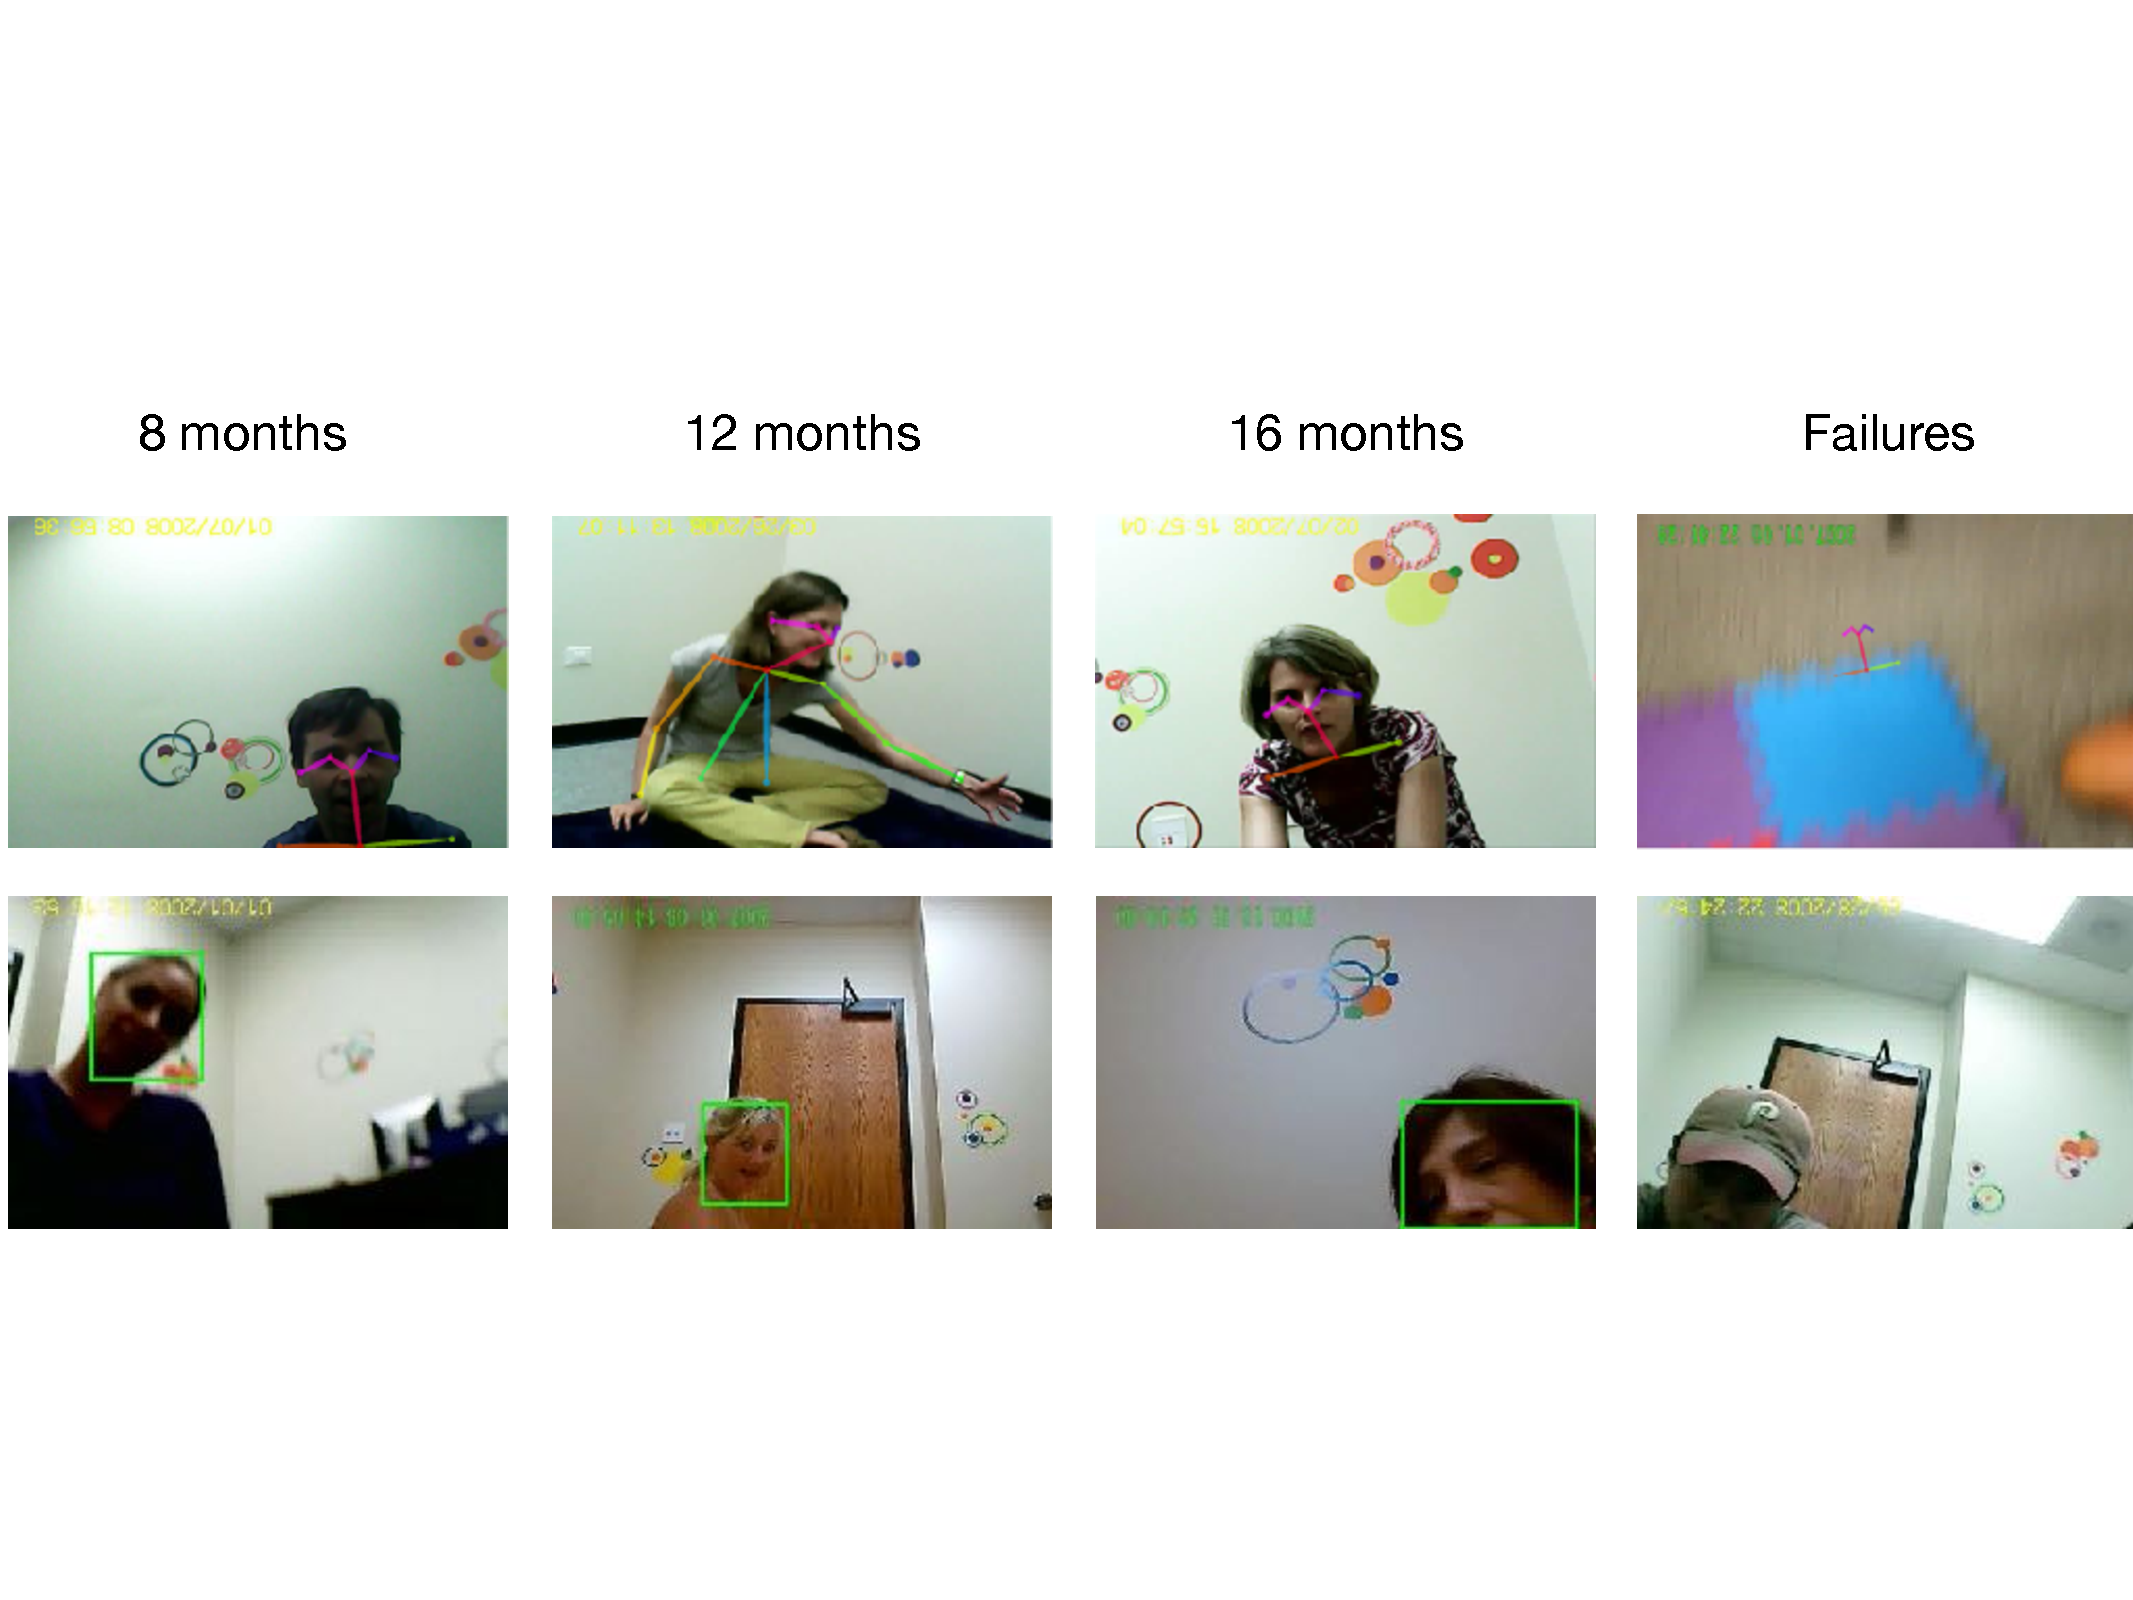
\includegraphics[width=5.5in]{images/detector_samples_banner.pdf}
\caption{\label{fig:frames} Example face and pose detections made by OpenPose (top row) and MTCNN (bottom row) from a child in each age group. The last column features a false positive from OpenPose and a false negative from MTCNN.}
\end{figure*}

\subsubsection{Algorithms}\label{algorithms}

The first face detection system made use of a series of Haar
feature-based cascade classifiers (Viola \& Jones, 2004) applied to each
individual frame. The second algorithm (based on work by K. Zhang et al.
(2016)) uses multi-task cascaded convolutional neural networks (MTCNNs)
for joint face detection and alignment, built to perform well in
real-world environments where varying illuminations and occlusions are
present. We used a Tensorflow implementation of this algorithm avaliable
at \url{https://github.com/davidsandberg/facenet}.

The CNN-based pose detector (OpenPose; Cao et al., 2017; Simon, Joo,
Matthews, \& Sheikh, 2017; Wei, Ramakrishna, Kanade, \& Sheikh, 2016))
provided the locations of 18 body parts (ears, nose, wrists, etc.) and
is available at
\url{https://github.com/CMU-Perceptual-Computing-Lab/openpose}. The
system uses a CNN for initial anatomical detection and subsequently
applies part affinity fields (PAFs) for part association, producing a
series of body part candidates. The candidates are then matched to a
single individual and finally assembled into a pose; here, we only made
use of the body parts relevant to the face and hands (nose and wrists).

\subsubsection{Detector evaluation}\label{detector-evaluation}

To evaluate face detector performance, we hand-labeled a ``gold set'' of
labeled frames. To account for the relatively rare appearance of faces
in the dataset, we hand-labeled two types of samples: a sample
containing a high density of faces (half reported by MTCNN, half by
OpenPose) and a random sample from the remaining frames. Each sample was
comprised of an equal number of frames taken from each child's video.
For wrist detections, the ``gold set'' was constructed in the same
manner, except frames with a high density of wrists came only from
detections made by OpenPose. Faces were classified as present if at
least half of the face was showing; wrists were classified as present if
any part of the wrist was showing. Precision (hits / hits + false
alarms), recall (hits / hits + misses), and F-score (harmonic mean of
precision and recall) were calculated for all detectors and are reported
in Table 2.

For face detection, MTCNN outperformed OpenPose when taking into account
only the composite F-score (0.89 MTCNN vs.~0.83 OpenPose). Although
MTCNN and OpenPose performed comparably with the random sample, MTCNN
performed better on the high density sample (specifically looking at
precision), suggesting that OpenPose generated more false positives than
MTCNN. ViolaJones performed quite poorly relative to the other
detectors, especially with respect to the random sample. We thus use
MTCNN detections in the following analyses. For wrist detection,
OpenPose performed moderately well (F = 0.74) with relatively high
precision but low recall on the randomly sampled frames (see Table 2).
We thus analyze wrist detections, with the caveat that we are likely
underestimating the proportion of hands in the dataset.

\begin{table}[ht]
\centering
\begin{tabular}{rllrrr}
\hline
Algorithm & Sample\ Type & P & R & F \\ 
\hline
MTCNN-Faces & High density & 0.89 & 0.92 & \textbf{0.90} \\ 
MTCNN-Faces & Random & 0.94 & 0.62 & 0.75 \\ 
OpenPose-Faces & High density & 0.78 & 0.93 & 0.84 \\ 
OpenPose-Faces & Random & 0.72 & 0.80 & \textbf{0.76} \\ 
ViolaJones-Faces & High density & 0.96 & 0.44 & 0.60 \\ 
ViolaJones-Faces & Random & 0.44 & 0.38 & 0.41 \\ 
OpenPose-Wrists & High density & 0.66 & 1.00 & 0.79 \\ 
OpenPose-Wrists & Random & 0.88 & 0.29 & 0.43 \\ 
\hline
\end{tabular}
\caption{Detector performance on both high density samples (where proportion of targets detected was high) and random samples (where frames were randomly selected). P, R, and F denote precision, recall, and F-score, respectively. Scores in bold are the highest F-scores for each sample type.} 
\end{table}

\section{Results}\label{results}

\begin{CodeChunk}
\begin{figure}[h]

{\centering \includegraphics{figs/posture-1} 

}

\caption[Proportion of time that infants in each age group spent in each posture/orientation relative to their caregiver]{Proportion of time that infants in each age group spent in each posture/orientation relative to their caregiver.}\label{fig:posture}
\end{figure}
\end{CodeChunk}

\subsection{Changes in Posture and
Orientation}\label{changes-in-posture-and-orientation}

The proportion of time infants spent sitting decreased with age, and the
proportion of time infants spent standing increased with age. Both
8-month-olds and 12-month-olds spent equivalent amounts of time
lying/crawling, which was markedly decreased in the 16-month-olds, who
spent most of their time sitting or standing (see Figure
\ref{fig:posture}). We also observed changes in children's orientation
relative to their caregivers: the 8-month-olds spent more time with
their caregiver behind them supporting their sitting positions (see
Figure \ref{fig:posture}).

\subsection{Changes in Access to Faces and
Hands}\label{changes-in-access-to-faces-and-hands}

We examined the proportion of face and hand detections across age (see
Figure \ref{fig:detByAge}). We observed a slight U-shaped function in
face detections, such that 12-month-olds appeared to have visual access
to slightly fewer faces faces than 8 or 16-month-olds; conversely, hand
detections perhaps appeared to generally increase with age.

Age related effects were much smaller than postural and locomotive
changes on children's visual access to faces and hands. Children's
posture was a major factor both in how many faces and hands they saw
during the play session. Infants who were sitting saw more faces than
infants who were lying down or being carried, while infants who were
standing saw the most faces (Figure \ref{fig:detByPosOrient}, upper
panel); this same pattern was also true for hand detections. Children's
orientation also impacted their visual access to faces and hands:
children who were far away from their caregiver were more likely to see
faces/hands than children who were close to their caregiver (Figure
\ref{fig:detByPosOrient}, lower panel).

\begin{CodeChunk}
\begin{figure}[h]

{\centering \includegraphics{figs/detByAge-1} 

}

\caption[Proportion of faces detected by the MTCNN model (left) and wrists detected by the OpenPose model (right) as a function of child's age]{Proportion of faces detected by the MTCNN model (left) and wrists detected by the OpenPose model (right) as a function of child's age. Larger dots indicate children who had longer play sessions and thus for whom there was more data.}\label{fig:detByAge}
\end{figure}
\end{CodeChunk}

\begin{CodeChunk}
\begin{figure*}[h]

{\centering \includegraphics{figs/detByPosOrient-1} 

}

\caption[Proportion of face and wrist detections as a function of children's posture (top panel) and orientation (bottom panel), binned by the age of the participant]{Proportion of face and wrist detections as a function of children's posture (top panel) and orientation (bottom panel), binned by the age of the participant.}\label{fig:detByPosOrient}
\end{figure*}
\end{CodeChunk}

To formalize these observations, we fit two generalized linear
mixed-effect models for the proportion of faces and the proportion of
hands infants saw in each posture and orientation, with participant's
age, orientation, and posture as fixed effects and with random slopes
for infant's orientation. Random slopes for posture or interactions
between our fixed effects caused the models to fail to converge.

\begin{table}[ht]
\centering
\begin{tabular}{rrrrr}
  \hline
 & Estimate & Std. Error & z value & Pr($>$$|$z$|$) \\ 
  \hline
  \textbf{Faces} \\
Intercept & -5.78 & 0.33 & -17.55 & 0.000 \\ 
  Close & 2.09 & 0.31 & 6.70 & 0.000 \\ 
  Far & 2.58 & 0.34 & 7.54 & 0.000 \\ 
  Prone & -0.18 & 0.08 & -2.39 & 0.017 \\ 
  Sit & 1.00 & 0.07 & 13.54 & 0.000 \\ 
  Stand & 1.50 & 0.08 & 19.98 & 0.000 \\ 
  Age & 0.17 & 0.17 & 0.97 & 0.334 \\ 
  \hline
  \textbf{Hands} \\
  Intercept & -4.84 & 0.19 & -25.40 & 0.000 \\ 
  Close & 0.88 & 0.17 & 5.25 & 0.000 \\ 
  Far & 1.77 & 0.27 & 6.45 & 0.000 \\ 
  Prone & 0.58 & 0.10 & 5.73 & 0.000 \\ 
  Sit & 1.18 & 0.10 & 12.04 & 0.000 \\ 
  Stand & 1.01 & 0.10 & 10.22 & 0.000 \\ 
  Age & 0.14 & 0.10 & 1.40 & 0.161 \\ 
   \hline
\end{tabular}
\caption{Model coefficients from generalized linear models predicting the proportion of faces (upper panel) and wrists (lower panel) seen by children.} 
\end{table}

A summary of the coefficients of the models can be found in Table 2.
While infant's posture and orientation significantly impacted the
proportion of faces and hands that infants saw, age was not a
significant predictor in either model. Thus, these results suggest that
infants' visual access to social information is modulated by their
posture and orientation, which is in turn a function of their general
locomotor development.

\subsection{Access to Faces and Hands During Labeling
Events}\label{access-to-faces-and-hands-during-labeling-events}

Finally, we explored how face and hand detections changed during object
labeling events as a function of infants' posture and orientation. We
analyzed a four-second window around each labeling event (e.g., ``Look
at the {[}zem{]}!''); these labeling events were hand-annotated and
synchronized with the frame-by-frame face/hand detections. We found that
infants' posture and orientations modulated their visual access to faces
and hands during labeling events; infants who were sitting or standing
were more likely to have visual access to this social information (see
Figure \ref{fig:detByNaming}). However, we did not find that infants saw
particularly more faces or hands during naming events relative to
baseline (avg. difference in proportion of hands, 8 m.o. = 0, 12 m.o. =
-0.003, 16 m.o. = -0.014; avg. difference in proportion of faces, 8 m.o.
= 0.003, 12 m.o. = 0.01, 16 m.o. = 0.021).

\section{General Discussion}\label{general-discussion}

We used a head-mounted camera to explore how children's postural and
locomotor development affects their visual access to social information,
here operationalized as the presence of the faces and hands of their
caregiver. Children's posture and orientation towards their caregiver
changed systematically across age, and both of these factors influenced
the proportion of faces and hands that were available in the child's
visual field. This work suggests that motor development modulates how
infants experience their visual world and the social information in it:
Infants that are sitting and standing have a different view of their
world, the people in it, and the actions that are being performed.

\begin{CodeChunk}
\begin{figure}[H]

{\centering \includegraphics{figs/detByNaming-1} 

}

\caption[Proportion of face and hand detections around a naming instance ('Look, a Zem']{Proportion of face and hand detections around a naming instance ('Look, a Zem'; +/- 2 seconds around each utterance) as a function of infants' posture. Error bars represent non-parametric bootstrapped 95 percent confidence intervals.}\label{fig:detByNaming}
\end{figure}
\end{CodeChunk}

We created a situation in the lab in which the context of interaction
was tightly controlled, but as children grow and change, the activities
in which they engage with their caregivers also vary, leading to
differences in the distribution of contexts they experience. Thus, more
work is needed to understand how our results relate to children's home
experiences (Fausey et al., 2016). The ability to walk is part of a
cascade of changes in children's experience, and our study captures only
a cross-sectional slice of this broader, multifaceted trajectory.

Understanding these changes has been a persistent challenge for
developmental psychology, but the field of computer vision has advanced
dramatically in recent years, creating a new generation of algorithmic
tools. These tools deal better with noisier, more complicated datasets
and extract richer and more detailed information than previous systems.
We hope that these new tools can be leveraged to understand the changing
infant perspective on the visual world and the implications of these
changes for linguistic, cognitive, and social development.

\section{Acknowledgements}\label{acknowledgements}

Thanks to Kaia Simmons, Kathy Woo, and Aditi Maliwal for help in
recruitment, data collection, and annotation. An earlier version of this
work was presented to the Cognitive Science Society in Frank et al.
(2013).

\section{References}\label{references}

\setlength{\parindent}{-0.1in} \setlength{\leftskip}{0.125in} \noindent

\hypertarget{refs}{}
\hypertarget{ref-adolph2006motor}{}
Adolph, K. E., \& Berger, S. E. (2006). Motor development.
\emph{Handbook of Child Psychology}.

\hypertarget{ref-adolph2012toward}{}
Adolph, K. E., Gilmore, R. O., Freeman, C., Sanderson, P., \& Millman,
D. (2012). Toward open behavioral science. \emph{Psychological Inquiry},
\emph{23}(3), 244--247.

\hypertarget{ref-bambach2017}{}
Bambach, S., Crandall, D. J., Smith, L. B., \& Yu, C. (2017). An
egocentric perspective on active vision and visual object learning in
toddlers. In \emph{Proceedings of the seventh joint ieee conference on
development and learning and on epigenetic robotics}.

\hypertarget{ref-cao2017realtime}{}
Cao, Z., Simon, T., Wei, S.-E., \& Sheikh, Y. (2017). Realtime
multi-person 2D pose estimation using part affinity fields. In
\emph{CVPR}.

\hypertarget{ref-clerkin2017}{}
Clerkin, E. M., Hart, E., Rehg, J. M., Yu, C., \& Smith, L. B. (2017).
Real-world visual statistics and infants' first-learned object names.
\emph{Phil. Trans. R. Soc. B}, \emph{372}(1711), 20160055.

\hypertarget{ref-csibra2009natural}{}
Csibra, G., \& Gergely, G. (2009). Natural pedagogy. \emph{Trends in
Cognitive Sciences}, \emph{13}(4), 148--153.

\hypertarget{ref-cummings1988}{}
Cummings, M., Van Hof-Van Duin, J., Mayer, D., Hansen, R., \& Fulton, A.
(1988). Visual fields of young children. \emph{Behavioural and Brain
Research}, \emph{29}(1), 7--16.

\hypertarget{ref-farroni2002eye}{}
Farroni, T., Csibra, G., Simion, F., \& Johnson, M. H. (2002). Eye
contact detection in humans from birth. \emph{Proceedings of the
National Academy of Sciences}, \emph{99}(14), 9602--9605.

\hypertarget{ref-fausey2016}{}
Fausey, C. M., Jayaraman, S., \& Smith, L. B. (2016). From faces to
hands: Changing visual input in the first two years. \emph{Cognition},
\emph{152}, 101--107.

\hypertarget{ref-franchak2011}{}
Franchak, J. M., Kretch, K. S., Soska, K. C., \& Adolph, K. E. (2011).
Head-mounted eye tracking: A new method to describe infant looking.
\emph{Child Development}, \emph{82}(6), 1738--1750.

\hypertarget{ref-frank2014visual}{}
Frank, M. C., Amso, D., \& Johnson, S. P. (2014). Visual search and
attention to faces during early infancy. \emph{Journal of Experimental
Child Psychology}, \emph{118}, 13--26.

\hypertarget{ref-frank2013}{}
Frank, M. C., Simmons, K., Yurovsky, D., \& Pusiol, G. (2013).
Developmental and postural changes in children’s visual access to faces.
In \emph{Proceedings of the 35th annual meeting of the cognitive science
society} (pp. 454--459).

\hypertarget{ref-frank2012measuring}{}
Frank, M. C., Vul, E., \& Saxe, R. (2012). Measuring the development of
social attention using free-viewing. \emph{Infancy}, \emph{17}(4),
355--375.

\hypertarget{ref-gredeback2010development}{}
Gredebäck, G., Fikke, L., \& Melinder, A. (2010). The development of
joint visual attention: A longitudinal study of gaze following during
interactions with mothers and strangers. \emph{Developmental Science},
\emph{13}(6), 839--848.

\hypertarget{ref-iverson2010}{}
Iverson, J. M. (2010). Developing language in a developing body: The
relationship between motor development and language development.
\emph{Journal of Child Language}, \emph{37}(2), 229--261.

\hypertarget{ref-karasik2014}{}
Karasik, L. B., Tamis-LeMonda, C. S., \& Adolph, K. E. (2014). Crawling
and walking infants elicit different verbal responses from mothers.
\emph{Developmental Science}, \emph{17}(3), 388--395.

\hypertarget{ref-kretch2014}{}
Kretch, K. S., Franchak, J. M., \& Adolph, K. E. (2014). Crawling and
walking infants see the world differently. \emph{Child Development},
\emph{85}(4), 1503--1518.

\hypertarget{ref-mayer1988}{}
Mayer, D., Fulton, A., \& Cummings, M. (1988). Visual fields of infants
assessed with a new perimetric technique. \emph{Investigative
Ophthalmology \& Visual Science}, \emph{29}(3), 452--459.

\hypertarget{ref-meltzoff2007like}{}
Meltzoff, A. N. (2007). ``Like me'': A foundation for social cognition.
\emph{Developmental Science}, \emph{10}(1), 126--134.

\hypertarget{ref-scheirer2014perceptual}{}
Scheirer, W. J., Anthony, S. E., Nakayama, K., \& Cox, D. D. (2014).
Perceptual annotation: Measuring human vision to improve computer
vision. \emph{IEEE Transactions on Pattern Analysis and Machine
Intelligence}, \emph{36}(8), 1679--1686.

\hypertarget{ref-simon2017hand}{}
Simon, T., Joo, H., Matthews, I., \& Sheikh, Y. (2017). Hand keypoint
detection in single images using multiview bootstrapping. In
\emph{CVPR}.

\hypertarget{ref-viola2004robust}{}
Viola, P., \& Jones, M. J. (2004). Robust real-time face detection.
\emph{International Journal of Computer Vision}, \emph{57}(2), 137--154.

\hypertarget{ref-walle2014}{}
Walle, E. A., \& Campos, J. J. (2014). Infant language development is
related to the acquisition of walking. \emph{Developmental Psychology},
\emph{50}(2), 336.

\hypertarget{ref-wei2016cpm}{}
Wei, S.-E., Ramakrishna, V., Kanade, T., \& Sheikh, Y. (2016).
Convolutional pose machines. In \emph{CVPR}.

\hypertarget{ref-yoshida2008}{}
Yoshida, H., \& Smith, L. (2008). What's in view for toddlers? Using a
head camera to study visual experience. \emph{Infancy}, \emph{13},
229--248.

\hypertarget{ref-yurovsky2012}{}
Yurovsky, D., Smith, L., \& Yu, C. (in press). Statistical word learning
at scale: The baby's view is better. \emph{Developmental Science}.

\hypertarget{ref-zhang2016}{}
Zhang, K., Zhang, Z., Li, Z., \& Qiao, Y. (2016). Joint face detection
and alignment using multitask cascaded convolutional networks.
\emph{IEEE Signal Processing Letters}, \emph{23}(10), 1499--1503.

\end{document}
